% Titelseite
\DeclareNewLayer[background,%
  width=115mm,%
  height=158mm,%
  hoffset=5mm,%
  voffset=10mm,%
  contents={%
    \resizebox{115mm}{!}{
\definecolor{cffffff}{RGB}{255,255,255}
\definecolor{c5b5a5a}{RGB}{91,90,90}
\definecolor{cee7f04}{RGB}{238,127,4}
\definecolor{c727272}{RGB}{114,114,114}


\def \globalscale {1.000000}
\begin{tikzpicture}[y=0.80pt, x=0.80pt, yscale=-\globalscale, xscale=\globalscale, inner sep=0pt, outer sep=0pt]
  \path[fill=cffffff,opacity=0.990,line join=miter,line cap=butt,miter
    limit=4.00,line width=3.351pt,rounded corners=0.0000cm] (0.0000,0.0000)
    rectangle (434.6457,597.1653);



\begin{scope}[shift={(0,-1002.8347)}]
\end{scope}
\begin{scope}[shift={(0,-1002.8347)}]
  \begin{scope}[cm={{0.19709,0.0,0.0,0.19709,(65.36527,901.74759)}}]
    \path[fill=c5b5a5a,line width=1.067pt] (680.3555,1963.3926) .. controls
      (679.3591,1963.4026) and (678.3189,1963.4486) .. (677.2324,1963.5391) ..
      controls (670.6642,1964.0838) and (669.1211,1964.7823) .. (665.3203,1968.9297)
      .. controls (659.2347,1975.5703) and (657.8482,1982.1074) ..
      (658.3574,2001.7637) .. controls (658.7173,2015.6535) and (659.2751,2019.5017)
      .. (661.5742,2023.9082) .. controls (665.4926,2031.4183) and
      (671.6228,2035.2422) .. (679.7441,2035.2422) .. controls (686.7201,2035.2422)
      and (690.2956,2033.9098) .. (695.1269,2029.5098) -- (698.1269,2026.7773) --
      (698.1169,2033.3438) .. controls (698.1129,2036.9548) and (697.4771,2042.1903)
      .. (696.7029,2044.9785) .. controls (693.5769,2056.2354) and
      (677.6017,2058.7760) .. (667.7830,2049.5781) .. controls (664.8223,2046.8047)
      and (664.7422,2046.8011) .. (662.8845,2049.3340) .. controls
      (661.2355,2051.5824) and (661.2777,2052.2278) .. (663.2263,2054.4297) ..
      controls (664.4537,2055.8166) and (667.8594,2058.0534) .. (670.7927,2059.4004)
      .. controls (682.6428,2064.8419) and (697.1001,2061.0920) ..
      (702.1072,2051.2773) .. controls (704.6243,2046.3433) and (704.7927,2043.4741)
      .. (704.7927,2005.2949) -- (704.7927,1964.5762) -- (701.4587,1964.5762) ..
      controls (698.6121,1964.5762) and (698.1248,1965.1863) .. (698.1248,1968.7559)
      -- (698.1248,1972.9355) -- (695.5037,1969.6016) .. controls
      (692.1456,1965.3325) and (687.3297,1963.3411) .. (680.3552,1963.3926) --
      cycle(681.6992,1970.0996) .. controls (685.9886,1970.2010) and
      (690.3675,1972.0710) .. (693.7910,1975.8066) -- (698.1250,1980.5352) --
      (698.1250,1998.6836) .. controls (698.1250,2019.0676) and (696.8966,2022.9557)
      .. (689.3164,2026.5527) .. controls (680.5243,2030.7249) and
      (670.8842,2027.4394) .. (667.3535,2019.0664) .. controls (664.4343,2012.1434)
      and (664.7623,1983.9065) .. (667.8281,1978.2637) .. controls
      (670.8179,1972.7609) and (676.1843,1969.9692) .. (681.6992,1970.0996) --
      cycle;



    \path[fill=c5b5a5a,line width=1.067pt] (721.1309,2049.7140) .. controls
      (719.9827,2048.5657) and (720.2477,2046.9226) .. (722.1976,2043.1004) ..
      controls (723.9204,2039.7236) and (724.7921,2035.3088) .. (724.7921,2029.9616)
      -- (724.7921,2021.9085) -- (728.7921,2021.9085) -- (732.7921,2021.9085) --
      (732.7921,2030.0614) .. controls (732.7921,2036.3657) and (731.9883,2039.6912)
      .. (729.2469,2044.7281) .. controls (725.6405,2051.3541) and
      (723.8631,2052.4461) .. (721.1309,2049.7140) -- cycle;



    \path[fill=c5b5a5a,line width=1.067pt] (427.0586,1963.2461) .. controls
      (418.2810,1963.2361) and (413.2756,1965.3640) .. (408.3984,1971.1602) ..
      controls (403.0942,1977.4639) and (401.5020,1983.9476) .. (401.5020,1999.2422)
      .. controls (401.5020,2007.4039) and (402.2360,2015.3408) ..
      (403.2617,2018.2754) .. controls (405.5342,2024.7773) and (410.9187,2031.1284)
      .. (416.0586,2033.3672) .. controls (425.4084,2037.4397) and
      (441.9198,2034.5833) .. (447.4336,2027.9395) .. controls (448.9509,2026.1113)
      and (448.9072,2025.4521) .. (447.1523,2023.6973) .. controls
      (445.2712,2021.8162) and (444.6870,2021.9057) .. (440.9746,2024.6504) ..
      controls (434.7391,2029.2605) and (424.1311,2029.7225) .. (418.1250,2025.6445)
      .. controls (412.2113,2021.6292) and (409.7674,2016.5840) ..
      (409.0449,2006.9082) -- (408.4707,1999.2422) -- (429.4902,1999.2422) --
      (450.5098,1999.2422) -- (449.7676,1989.4160) .. controls (448.3941,1971.2549)
      and (441.4522,1963.2561) .. (427.0586,1963.2461) -- cycle(425.7988,1969.8027)
      .. controls (428.4804,1969.7727) and (431.3100,1970.4520) ..
      (434.1523,1971.9219) .. controls (438.9428,1974.3992) and (440.6789,1977.5046)
      .. (442.0215,1985.9980) -- (443.0605,1992.5762) -- (425.7559,1992.5762) --
      (408.4512,1992.5762) -- (409.3477,1986.9707) .. controls (411.0446,1976.3589)
      and (417.7540,1969.8920) .. (425.7988,1969.8027) -- cycle;



    \path[fill=c5b5a5a,line width=1.067pt] (492.7930,1935.2422) --
      (492.7930,1984.5762) -- (492.7930,2033.9082) -- (496.1250,2033.9082) ..
      controls (498.7917,2033.9082) and (499.4590,2033.2428) .. (499.4590,2030.5762)
      .. controls (499.4590,2027.1467) and (501.2822,2026.1317) ..
      (502.8594,2028.6836) .. controls (503.3493,2029.4764) and (505.6342,2031.2733)
      .. (507.9375,2032.6777) .. controls (513.5594,2036.1055) and
      (524.0687,2036.0799) .. (529.7383,2032.6227) .. controls (532.0920,2031.1875)
      and (535.3927,2027.4401) .. (537.0723,2024.2946) .. controls
      (539.8518,2019.0894) and (540.1250,2016.8387) .. (540.1250,1999.2419) ..
      controls (540.1250,1981.6452) and (539.8518,1979.3945) .. (537.0723,1974.1892)
      .. controls (532.9143,1966.4024) and (527.3772,1963.2558) ..
      (517.8379,1963.2458) .. controls (511.2120,1963.2458) and (509.6039,1963.7824)
      .. (505.5059,1967.3806) -- (500.7930,1971.5173) -- (500.7930,1953.3806) --
      (500.7930,1935.2419) -- (496.7930,1935.2419) -- cycle(516.8418,1969.9082) ..
      controls (522.7117,1969.9222) and (528.1109,1973.1280) .. (530.8828,1978.8496)
      .. controls (532.7682,1982.7412) and (533.3485,1987.1382) ..
      (533.3965,1997.9082) .. controls (533.4744,2015.4056) and (530.9455,2023.2490)
      .. (524.1934,2026.4531) .. controls (518.7978,2029.0135) and
      (514.8328,2029.0695) .. (509.2969,2026.6602) .. controls (501.6519,2023.3329)
      and (500.7930,2020.6601) .. (500.7930,2000.2129) .. controls
      (500.7930,1979.6951) and (501.9930,1975.4247) .. (508.7480,1971.9316) ..
      controls (511.4080,1970.5561) and (514.1736,1969.9018) .. (516.8418,1969.9082)
      -- cycle;



    \path[fill=c5b5a5a,line width=1.067pt] (566.3786,2032.5410) .. controls
      (558.7150,2027.8686) and (557.6537,2023.2812) .. (557.0557,1992.2418) --
      (556.5227,1964.5752) -- (560.6574,1964.5752) -- (564.7921,1964.5752) --
      (564.7921,1990.7070) .. controls (564.7921,2019.7936) and (565.7967,2024.3442)
      .. (572.8635,2027.2714) .. controls (577.2419,2029.0850) and
      (584.1739,2028.1932) .. (588.3309,2025.2815) .. controls (594.4412,2021.0017)
      and (595.4588,2015.8753) .. (595.4588,1989.3737) -- (595.4588,1964.5752) --
      (598.7921,1964.5752) -- (602.1255,1964.5752) -- (602.1255,1999.2418) --
      (602.1255,2033.9085) -- (598.7921,2033.9085) .. controls (596.0675,2033.9085)
      and (595.4588,2033.2573) .. (595.4588,2030.3428) -- (595.4588,2026.7770) --
      (592.4588,2029.5095) .. controls (587.6446,2033.8944) and (584.0569,2035.2422)
      .. (577.2131,2035.2368) .. controls (573.1271,2035.2368) and
      (569.1872,2034.2534) .. (566.3786,2032.5410) -- cycle;



    \path[fill=c5b5a5a,line width=1.067pt] (902.9203,2033.5005) .. controls
      (901.4565,2032.4300) and (900.7161,2030.5035) .. (900.9988,2028.5005) ..
      controls (901.3867,2025.7528) and (902.1906,2025.2418) .. (906.1255,2025.2418)
      .. controls (910.0604,2025.2418) and (910.8643,2025.7528) ..
      (911.2521,2028.5005) .. controls (911.6605,2031.3941) and (908.7344,2035.2418)
      .. (906.1255,2035.2418) .. controls (905.6725,2035.2418) and
      (904.2301,2034.4582) .. (902.9203,2033.5005) -- cycle;



    \path[fill=c5b5a5a,line width=1.067pt] (1122.1864,2033.3152) .. controls
      (1121.3070,2032.2556) and (1120.7835,2030.0056) .. (1121.0232,2028.3152) ..
      controls (1121.3833,2025.7747) and (1122.2679,2025.2418) ..
      (1126.1255,2025.2418) .. controls (1130.0604,2025.2418) and
      (1130.8643,2025.7528) .. (1131.2521,2028.5005) .. controls
      (1132.0037,2033.8253) and (1125.4836,2037.2881) .. (1122.1864,2033.3152) --
      cycle;



    \path[fill=c5b5a5a,line width=1.067pt] (1293.7676,1963.2969) .. controls
      (1289.3770,1963.3399) and (1285.0441,1964.1493) .. (1282.1055,1965.7109) ..
      controls (1276.6655,1968.6017) and (1271.4590,1975.6405) ..
      (1271.4590,1980.1055) .. controls (1271.4590,1984.6423) and
      (1277.7374,1984.5831) .. (1278.8789,1980.0355) .. controls
      (1281.3428,1970.2185) and (1297.3445,1966.4621) .. (1304.8262,1973.9437) ..
      controls (1306.9076,1976.0251) and (1307.4590,1978.3909) ..
      (1307.4590,1985.2425) -- (1307.4590,1993.9085) -- (1297.1250,1993.9375) ..
      controls (1278.3577,1993.9905) and (1270.0799,2000.7872) ..
      (1270.1719,2016.0664) .. controls (1270.2259,2025.0036) and
      (1271.9667,2028.9324) .. (1277.5488,2032.7246) -- (1277.5488,2032.7246) ..
      controls (1280.6611,2034.8385) and (1283.1461,2035.2880) ..
      (1289.7285,2034.9199) .. controls (1296.6871,2034.5307) and
      (1298.8534,2033.7685) .. (1303.3945,2030.1191) -- (1308.7930,2025.7832) --
      (1308.7930,2029.8457) .. controls (1308.7930,2033.3887) and
      (1309.2615,2033.9101) .. (1312.4590,2033.9101) -- (1316.1250,2033.9101) --
      (1315.6973,2006.2421) .. controls (1315.2037,1974.3072) and
      (1314.0066,1969.3863) .. (1305.7715,1965.4785) .. controls
      (1302.6065,1963.9766) and (1298.1582,1963.2519) .. (1293.7676,1963.2949) --
      cycle(1307.4590,1999.2422) -- (1307.4590,2008.9922) .. controls
      (1307.4590,2017.8923) and (1307.1398,2019.0473) .. (1303.7930,2022.2402) ..
      controls (1301.7763,2024.1641) and (1298.4355,2026.3763) ..
      (1296.3711,2027.1562) -- (1296.3711,2027.1562) .. controls
      (1285.2125,2031.3722) and (1275.9574,2024.7183) .. (1277.2969,2013.4433) ..
      controls (1278.4268,2003.9332) and (1286.0465,1999.2630) ..
      (1300.4590,1999.2480) -- cycle;



    \path[fill=c5b5a5a,line width=1.067pt] (304.7921,1987.2418) --
      (304.7921,1940.5752) -- (328.7921,1940.5752) -- (352.7921,1940.5752) --
      (352.7921,1943.9085) -- (352.7921,1947.2418) -- (332.1255,1947.2418) --
      (311.4588,1947.2418) -- (311.4588,1965.2418) -- (311.4588,1983.2418) --
      (329.4588,1983.2418) -- (347.4588,1983.2418) -- (347.4588,1986.5365) --
      (347.4588,1989.8311) -- (329.7921,1990.2031) -- (312.1255,1990.5752) --
      (311.7591,2012.2418) -- (311.3927,2033.9085) -- (308.0924,2033.9085) --
      (304.7921,2033.9085) -- cycle;



    \path[fill=c5b5a5a,line width=1.067pt] (366.1255,1999.2418) --
      (366.1255,1964.5752) -- (369.4588,1964.5752) .. controls (372.2818,1964.5752)
      and (372.7921,1965.1944) .. (372.7921,1968.6196) -- (372.7921,1972.6641) --
      (377.5032,1967.9529) .. controls (381.3123,1964.1439) and (383.2271,1963.2418)
      .. (387.5032,1963.2418) .. controls (392.4078,1963.2418) and
      (392.7921,1963.5133) .. (392.7921,1966.9776) .. controls (392.7921,1970.3494)
      and (392.3267,1970.7265) .. (388.0152,1970.8487) .. controls
      (384.9980,1970.9337) and (381.9877,1972.1368) .. (379.8434,1974.1130) ..
      controls (373.5971,1979.8697) and (372.7921,1983.9514) .. (372.7921,2009.8657)
      -- (372.7921,2033.9085) -- (369.4588,2033.9085) -- (366.1255,2033.9085) --
      cycle;



    \path[fill=c5b5a5a,line width=1.067pt] (466.1255,1999.2418) --
      (466.1255,1964.5752) -- (469.4588,1964.5752) -- (472.7921,1964.5752) --
      (472.7921,1999.2418) -- (472.7921,2033.9085) -- (469.4588,2033.9085) --
      (466.1255,2033.9085) -- cycle;



    \path[fill=c5b5a5a,line width=1.067pt] (620.7921,1999.2418) --
      (620.7921,1964.5752) -- (624.7921,1964.5752) .. controls (628.3170,1964.5752)
      and (628.7921,1965.0344) .. (628.7921,1968.4418) -- (628.7921,1972.3085) --
      (633.3255,1967.7752) .. controls (637.0068,1964.0939) and (638.8863,1963.2418)
      .. (643.3255,1963.2418) .. controls (648.4247,1963.2418) and
      (648.7921,1963.4929) .. (648.7921,1966.9776) .. controls (648.7921,1970.3381)
      and (648.3200,1970.7267) .. (644.0914,1970.8466) .. controls
      (638.0061,1971.0191) and (633.7330,1973.8995) .. (630.9914,1979.6768) ..
      controls (629.1929,1983.4670) and (628.7921,1988.8302) .. (628.7921,2009.1100)
      -- (628.7921,2033.9085) -- (624.7921,2033.9085) -- (620.7921,2033.9085) --
      cycle;



    \path[fill=c5b5a5a,line width=1.067pt] (802.1255,1991.9415) --
      (802.1255,1949.9745) -- (799.1255,1951.1570) .. controls (797.4755,1951.8074)
      and (792.6755,1953.8850) .. (788.4588,1955.7739) -- (780.7921,1959.2082) --
      (780.7921,1955.4035) .. controls (780.7921,1951.4932) and (782.9137,1950.2064)
      .. (804.4588,1941.0480) -- (808.7921,1939.2060) -- (808.7921,1986.5573) --
      (808.7921,2033.9085) -- (805.4588,2033.9085) -- (802.1255,2033.9085) -- cycle;



    \path[fill=c5b5a5a,line width=1.067pt] (866.1255,1991.9255) --
      (866.1255,1949.9423) -- (858.4588,1953.3766) .. controls (844.2666,1959.7341)
      and (844.7921,1959.6574) .. (844.7921,1955.3722) .. controls
      (844.7921,1951.8345) and (845.7019,1951.1741) .. (857.7921,1945.9352) ..
      controls (864.9421,1942.8370) and (871.5421,1939.9994) .. (872.4588,1939.6294)
      .. controls (873.7735,1939.0987) and (874.1255,1948.9820) ..
      (874.1255,1986.4327) -- (874.1255,2033.9085) -- (870.1255,2033.9085) --
      (866.1255,2033.9085) -- (866.1255,1991.9253) -- cycle;



    \path[fill=c5b5a5a,line width=1.067pt] (1014.1255,1992.7975) .. controls
      (1014.1255,1970.1864) and (1013.7802,1951.3412) .. (1013.3583,1950.9192) ..
      controls (1012.9363,1950.4973) and (1008.0981,1952.1995) ..
      (1002.6067,1954.7020) -- (992.6224,1959.2520) -- (993.0406,1955.1676) ..
      controls (993.4229,1951.4341) and (994.4325,1950.6528) ..
      (1004.7921,1946.0741) .. controls (1011.0255,1943.3190) and
      (1017.1755,1940.6736) .. (1018.4588,1940.1953) .. controls
      (1020.6535,1939.3773) and (1020.7921,1942.1353) .. (1020.7921,1986.6172) --
      (1020.7921,2033.9086) -- (1017.4588,2033.9086) -- (1014.1255,2033.9086) --
      cycle;



    \path[fill=c5b5a5a,line width=1.067pt] (1091.1055,1940.5762) .. controls
      (1086.8023,1940.5762) and (1086.5454,1940.9470) .. (1069.1055,1972.4590) ..
      controls (1059.4003,1989.9954) and (1051.4590,2005.5967) ..
      (1051.4590,2007.1270) .. controls (1051.4590,2009.8103) and
      (1052.0985,2009.9082) .. (1069.4590,2009.9082) -- (1087.4590,2009.9082) --
      (1087.4590,2021.9082) -- (1087.4590,2033.9082) -- (1091.4590,2033.9082) --
      (1095.4590,2033.9082) -- (1095.4590,2021.9082) -- (1095.4590,2009.9082) --
      (1101.4590,2009.9082) .. controls (1106.9701,2009.9082) and
      (1107.4590,2009.6379) .. (1107.4590,2006.5762) .. controls
      (1107.4590,2003.5144) and (1106.9701,2003.2422) .. (1101.4590,2003.2422) --
      (1095.4590,2003.2422) -- (1095.4590,1971.9082) -- (1095.4590,1940.5762) --
      cycle(1086.4043,1955.3535) .. controls (1087.2841,1955.5796) and
      (1087.4590,1961.0058) .. (1087.4590,1978.2793) -- (1087.4590,2003.2422) --
      (1074.1250,2003.2422) .. controls (1066.7917,2003.2422) and
      (1060.7930,2002.8675) .. (1060.7930,2002.4102) .. controls
      (1060.7930,2001.4124) and (1083.1303,1959.7007) .. (1085.6758,1955.9453) ..
      controls (1085.9605,1955.5253) and (1086.2013,1955.3013) ..
      (1086.4043,1955.3535) -- cycle;



    \path[fill=c5b5a5a,line width=1.067pt] (1175.4588,1987.1613) --
      (1175.4588,1940.4142) -- (1180.4395,1940.8280) -- (1185.4202,1941.2418) --
      (1198.7861,1980.1439) .. controls (1206.1373,2001.5401) and
      (1212.5193,2019.4134) .. (1212.9683,2019.8624) .. controls
      (1213.4173,2020.3114) and (1218.0867,2008.2054) .. (1223.3448,1992.9603) ..
      controls (1228.6029,1977.7151) and (1234.8296,1959.6948) ..
      (1237.1819,1952.9150) -- (1241.4588,1940.5882) -- (1246.4588,1940.5782) --
      (1251.4588,1940.5682) -- (1251.4588,1987.2349) -- (1251.4588,2033.9016) --
      (1248.1453,2033.9016) -- (1244.8318,2033.9016) -- (1244.4787,1994.4385) --
      (1244.1255,1954.9753) -- (1230.2579,1994.5076) .. controls
      (1212.0264,2046.4799) and (1214.4777,2046.4592) .. (1196.3097,1994.7954) --
      (1182.7922,1956.3561) -- (1182.4387,1995.1290) -- (1182.0852,2033.9019) --
      (1178.7720,2033.9019) -- (1175.4588,2033.9019) -- cycle;



    \path[fill=c5b5a5a,line width=1.067pt] (1334.1255,1999.2418) --
      (1334.1255,1964.5752) -- (1338.1255,1964.5752) .. controls
      (1341.6504,1964.5752) and (1342.1255,1965.0344) .. (1342.1255,1968.4418) --
      (1342.1255,1972.3085) -- (1346.6588,1967.7752) .. controls
      (1350.3401,1964.0939) and (1352.2196,1963.2418) .. (1356.6588,1963.2418) ..
      controls (1361.7581,1963.2418) and (1362.1255,1963.4929) ..
      (1362.1255,1966.9776) .. controls (1362.1255,1970.3064) and
      (1361.6354,1970.7272) .. (1357.6267,1970.8409) .. controls
      (1351.2337,1971.0221) and (1347.8596,1973.2291) .. (1344.7965,1979.2333) ..
      controls (1342.4084,1983.9145) and (1342.1255,1987.0868) ..
      (1342.1255,2009.1887) -- (1342.1255,2033.9085) -- (1338.1255,2033.9085) --
      (1334.1255,2033.9085) -- cycle;



    \path[fill=c5b5a5a,line width=1.067pt] (1371.4588,2030.6767) .. controls
      (1371.4588,2028.8591) and (1378.9829,2015.2933) .. (1388.6525,1999.6767) --
      (1405.8463,1971.9085) -- (1389.3192,1971.5353) -- (1372.7922,1971.1622) --
      (1372.7922,1967.8687) -- (1372.7922,1964.5752) -- (1394.1255,1964.5752) ..
      controls (1414.9306,1964.5752) and (1415.4588,1964.6452) ..
      (1415.4588,1967.3843) .. controls (1415.4588,1968.9293) and
      (1407.6588,1982.7788) .. (1398.1255,1998.1610) .. controls
      (1388.5922,2013.5432) and (1380.7922,2026.3791) .. (1380.7922,2026.6852) ..
      controls (1380.7922,2026.9914) and (1389.1922,2027.2418) ..
      (1399.4588,2027.2418) -- (1418.1255,2027.2418) -- (1418.1255,2030.5752) --
      (1418.1255,2033.9085) -- (1394.7922,2033.9085) -- (1371.4588,2033.9085) --
      cycle;



    \path[fill=c5b5a5a,line width=1.067pt] (924.7921,1986.5752) --
      (924.7921,1983.2418) -- (952.1255,1983.2418) -- (979.4588,1983.2418) --
      (979.4588,1986.5752) -- (979.4588,1989.9085) -- (952.1255,1989.9085) --
      (924.7921,1989.9085) -- cycle;



    \path[fill=c5b5a5a,line width=1.067pt] (466.8497,1948.1155) .. controls
      (465.4498,1947.0918) and (464.7202,1945.1412) .. (464.9988,1943.1671) ..
      controls (465.3700,1940.5375) and (466.2310,1939.9085) .. (469.4588,1939.9085)
      .. controls (472.8066,1939.9085) and (473.5262,1940.4918) ..
      (473.8720,1943.4855) .. controls (474.3956,1948.0170) and (470.3567,1950.6799)
      .. (466.8497,1948.1155) -- cycle;



    \path[fill=c5b5a5a,line width=1.067pt] (1277.3369,1946.7382) .. controls
      (1275.6422,1942.3220) and (1277.3369,1939.9085) .. (1282.1438,1939.9085) ..
      controls (1286.4198,1939.9085) and (1286.7922,1940.2290) ..
      (1286.7922,1943.9085) .. controls (1286.7922,1947.4485) and
      (1286.2928,1947.9566) .. (1282.4497,1948.3270) .. controls
      (1279.5215,1948.6092) and (1277.8563,1948.0917) .. (1277.3369,1946.7382) --
      cycle;



    \path[fill=c5b5a5a,line width=1.067pt] (1305.3369,1946.7382) .. controls
      (1303.6422,1942.3220) and (1305.3369,1939.9085) .. (1310.1438,1939.9085) ..
      controls (1314.4198,1939.9085) and (1314.7922,1940.2290) ..
      (1314.7922,1943.9085) .. controls (1314.7922,1947.4485) and
      (1314.2928,1947.9566) .. (1310.4497,1948.3270) .. controls
      (1307.5215,1948.6092) and (1305.8563,1948.0917) .. (1305.3369,1946.7382) --
      cycle;



    \path[fill=c5b5a5a,line width=1.067pt] (448.1250,1731.2422) .. controls
      (423.7092,1731.2422) and (406.5072,1744.4190) .. (399.9727,1768.1250) ..
      controls (396.4355,1780.9572) and (396.2826,1829.4645) .. (399.7441,1840.5762)
      .. controls (404.8576,1856.9903) and (416.1675,1869.6585) ..
      (429.9629,1874.4238) .. controls (439.0930,1877.5776) and (461.9886,1876.7507)
      .. (470.3594,1872.9648) .. controls (479.4611,1868.8483) and
      (488.2392,1860.1149) .. (492.7207,1850.7168) .. controls (498.5759,1838.4380)
      and (499.8627,1828.0076) .. (499.1250,1798.7988) .. controls
      (498.5750,1777.0222) and (498.0532,1772.0586) .. (495.5977,1765.2422) ..
      controls (487.3969,1742.4779) and (471.7085,1731.2422) .. (448.1250,1731.2422)
      -- cycle(448.1250,1755.9082) .. controls (455.9919,1755.9082) and
      (456.9980,1756.2527) .. (461.2793,1760.4023) .. controls (468.9011,1767.7897)
      and (470.4212,1776.1620) .. (469.8984,1807.9082) .. controls
      (469.5024,1831.9588) and (469.1727,1835.1931) .. (466.5488,1840.8730) ..
      controls (464.7795,1844.7031) and (461.9073,1848.2268) .. (459.2168,1849.8672)
      .. controls (456.3334,1851.6251) and (452.4700,1852.5645) ..
      (448.1250,1852.5645) .. controls (439.1598,1852.5645) and (433.4196,1848.9223)
      .. (429.7012,1840.8730) .. controls (427.0773,1835.1931) and
      (426.7496,1831.9588) .. (426.3535,1807.9082) .. controls (425.8307,1776.1620)
      and (427.3489,1767.7897) .. (434.9707,1760.4023) .. controls
      (439.2520,1756.2527) and (440.2581,1755.9082) .. (448.1250,1755.9082) --
      cycle;



    \path[fill=c5b5a5a,line width=1.067pt] (547.8402,1874.7116) .. controls
      (529.8717,1868.8697) and (518.5125,1855.3329) .. (516.1182,1836.9085) --
      (515.2086,1829.9085) -- (529.8286,1829.9085) -- (544.4486,1829.9085) --
      (545.3604,1836.7818) .. controls (547.0143,1849.2500) and (558.1019,1856.3351)
      .. (570.2595,1852.6925) .. controls (577.9142,1850.3991) and
      (580.2960,1845.5155) .. (579.6599,1833.4183) .. controls (579.3365,1827.2690)
      and (571.1814,1820.4063) .. (557.4588,1814.7357) .. controls
      (536.0695,1805.8969) and (524.4269,1795.3658) .. (520.6618,1781.4516) ..
      controls (518.5728,1773.7313) and (519.8114,1759.7133) .. (523.1625,1753.1509)
      .. controls (526.6341,1746.3524) and (535.2564,1738.4754) ..
      (543.2956,1734.7582) .. controls (548.4094,1732.3937) and (551.9560,1731.9085)
      .. (564.1255,1731.9085) .. controls (577.4776,1731.9085) and
      (579.4711,1732.2419) .. (586.3676,1735.6286) .. controls (599.0600,1741.8615)
      and (607.1998,1753.5973) .. (608.4586,1767.4786) -- (609.1625,1775.2418) --
      (595.1257,1775.2418) -- (581.0889,1775.2418) -- (580.1595,1770.2879) ..
      controls (578.1195,1759.4134) and (572.8107,1754.5149) .. (563.3345,1754.7634)
      .. controls (553.6619,1755.0170) and (548.7921,1760.6333) ..
      (548.7921,1771.5351) .. controls (548.7921,1776.1295) and (549.6025,1777.7589)
      .. (553.9395,1781.8846) .. controls (556.7705,1784.5777) and
      (562.6205,1788.1848) .. (566.9395,1789.9003) .. controls (590.9209,1799.4263)
      and (602.9900,1809.2990) .. (606.8389,1822.5386) .. controls
      (609.7046,1832.3965) and (609.0550,1848.4703) .. (605.4954,1855.7797) ..
      controls (602.0530,1862.8484) and (594.9512,1869.6805) .. (587.5780,1873.0166)
      .. controls (579.8030,1876.5345) and (556.5037,1877.5283) ..
      (547.8402,1874.7116) -- cycle;



    \path[fill=c5b5a5a,line width=1.067pt] (655.8402,1874.7116) .. controls
      (637.8257,1868.8547) and (626.4647,1855.2714) .. (624.2219,1836.9085) --
      (623.3669,1829.9085) -- (637.9078,1829.9085) -- (652.4486,1829.9085) --
      (653.3254,1836.5185) .. controls (654.8763,1848.2096) and (664.6254,1855.4872)
      .. (675.9017,1853.3718) .. controls (682.4724,1852.1391) and
      (686.0547,1848.7966) .. (687.4727,1842.5752) .. controls (690.3036,1830.1545)
      and (684.5251,1822.8594) .. (665.3875,1814.6935) .. controls
      (643.7553,1805.4633) and (632.3714,1795.1609) .. (628.6637,1781.4586) ..
      controls (626.5730,1773.7320) and (627.8102,1759.7155) .. (631.1625,1753.1509)
      .. controls (634.6341,1746.3524) and (643.2564,1738.4754) ..
      (651.2956,1734.7582) .. controls (656.4094,1732.3937) and (659.9560,1731.9085)
      .. (672.1255,1731.9085) .. controls (685.4776,1731.9085) and
      (687.4711,1732.2419) .. (694.3676,1735.6286) .. controls (707.0600,1741.8615)
      and (715.1998,1753.5973) .. (716.4586,1767.4786) -- (717.1625,1775.2418) --
      (703.1257,1775.2418) -- (689.0889,1775.2418) -- (688.1595,1770.2879) ..
      controls (687.6484,1767.5632) and (686.4328,1763.7920) .. (685.4582,1761.9074)
      .. controls (680.6698,1752.6475) and (664.8266,1752.0813) ..
      (659.4030,1760.9762) .. controls (655.7078,1767.0365) and (655.9661,1775.3984)
      .. (659.9948,1780.1395) .. controls (663.3222,1784.0553) and
      (666.2110,1785.6891) .. (687.6200,1795.7639) .. controls (708.6356,1805.6535)
      and (716.7921,1817.2507) .. (716.7921,1837.2418) .. controls
      (716.7921,1849.5029) and (713.9064,1857.7721) .. (707.2252,1864.6566) ..
      controls (698.9388,1873.1952) and (691.9741,1875.7177) .. (675.4588,1876.1618)
      .. controls (666.2609,1876.4092) and (659.5316,1875.9118) ..
      (655.8402,1874.7116) -- cycle;



    \path[fill=c5b5a5a,line width=1.067pt] (767.8910,1874.7336) .. controls
      (751.3705,1869.3366) and (740.1058,1855.9050) .. (736.0494,1836.7669) ..
      controls (733.5080,1824.7767) and (733.5080,1783.0398) .. (736.0494,1771.0496)
      .. controls (739.6038,1754.2802) and (747.1245,1743.2955) ..
      (759.7314,1736.4597) .. controls (768.0108,1731.9704) and (768.3531,1731.9082)
      .. (784.7921,1731.9082) .. controls (799.4579,1731.9082) and
      (802.2955,1732.2865) .. (808.4282,1735.0592) .. controls (821.2491,1740.8559)
      and (829.9740,1754.0741) .. (832.2364,1771.1289) -- (833.1357,1777.9083) --
      (818.9639,1777.9083) .. controls (808.1227,1777.9083) and (804.7921,1777.4951)
      .. (804.7921,1776.1503) .. controls (804.7921,1775.1834) and
      (803.8606,1771.2554) .. (802.7220,1767.4213) .. controls (800.1349,1758.7098)
      and (795.2294,1755.2516) .. (785.4588,1755.2516) .. controls
      (776.9414,1755.2516) and (771.1784,1758.6999) .. (767.1793,1766.1893) ..
      controls (764.2450,1771.6843) and (764.1255,1773.1364) .. (764.1255,1803.2750)
      .. controls (764.1255,1834.1170) and (764.1812,1834.7500) ..
      (767.4588,1841.1177) .. controls (771.7248,1849.4056) and (777.3620,1852.5750)
      .. (787.8375,1852.5750) .. controls (792.1799,1852.5750) and
      (797.3220,1851.6800) .. (799.5250,1850.5407) -- (803.4588,1848.5065) --
      (803.4588,1835.2076) -- (803.4588,1821.9085) -- (793.4588,1821.9085) --
      (783.4588,1821.9085) -- (783.4588,1811.2418) -- (783.4588,1800.5751) --
      (808.1505,1800.5751) -- (832.8422,1800.5751) -- (832.4838,1830.7914) --
      (832.1255,1861.0075) -- (824.7921,1865.9210) .. controls (812.6204,1874.0764)
      and (807.3050,1875.6086) .. (789.4588,1876.1064) .. controls
      (778.4544,1876.4134) and (771.7204,1875.9848) .. (767.8910,1874.7338) --
      cycle;



    \path[fill=c5b5a5a,line width=1.067pt] (932.9917,1873.9124) .. controls
      (925.1490,1871.0911) and (923.8388,1870.2570) .. (916.3436,1863.3135) ..
      controls (909.4427,1856.9207) and (904.6495,1847.1241) .. (903.7912,1837.6583)
      -- (903.0884,1829.9083) -- (917.2132,1829.9083) -- (931.3380,1829.9083) --
      (932.1392,1834.9083) .. controls (934.2623,1848.1572) and (939.5640,1853.1312)
      .. (951.6342,1853.1984) .. controls (958.3648,1853.2364) and
      (959.8821,1852.7521) .. (963.0921,1849.5447) .. controls (966.3013,1846.3381)
      and (966.7921,1844.8035) .. (966.7921,1837.9758) .. controls
      (966.7921,1825.6461) and (965.1570,1824.1124) .. (939.2529,1812.1451) ..
      controls (916.5144,1801.6402) and (907.0684,1789.6718) .. (906.9701,1771.2416)
      .. controls (906.8822,1754.7703) and (913.4862,1743.7415) ..
      (927.9701,1736.1710) .. controls (935.7660,1732.0961) and (936.8013,1731.9083)
      .. (951.4588,1731.9083) .. controls (965.5080,1731.9083) and
      (967.3504,1732.2057) .. (973.4588,1735.4597) .. controls (986.3857,1742.3461)
      and (994.1936,1753.6415) .. (996.1191,1768.2416) -- (997.0424,1775.2416) --
      (982.4262,1775.2416) -- (967.8099,1775.2416) -- (967.0653,1769.6904) ..
      controls (966.1051,1762.5309) and (962.4137,1757.6470) .. (956.4525,1755.6490)
      .. controls (946.5276,1752.3225) and (937.0036,1758.4594) ..
      (935.8220,1768.9424) .. controls (934.8005,1778.0052) and (939.8471,1782.7980)
      .. (961.3403,1793.1772) .. controls (981.0498,1802.6951) and
      (987.4313,1807.9967) .. (992.6070,1819.1529) .. controls (995.4182,1825.2123)
      and (996.0444,1828.5333) .. (996.0180,1837.2416) .. controls
      (995.9615,1855.8024) and (988.1517,1867.7976) .. (972.2499,1873.7472) ..
      controls (962.1246,1877.5356) and (943.2837,1877.6149) .. (932.9917,1873.9125)
      -- cycle;



    \path[fill=c5b5a5a,line width=1.067pt] (1180.9277,1731.2422) .. controls
      (1162.7170,1731.2422) and (1151.9635,1741.1233) .. (1146.5000,1762.8789) ..
      controls (1143.5273,1774.7160) and (1143.1309,1830.2315) ..
      (1145.9316,1842.4551) .. controls (1149.6736,1858.7869) and
      (1156.7575,1869.5342) .. (1166.7812,1874.0879) .. controls
      (1174.0966,1877.4107) and (1190.1770,1877.4010) .. (1197.5137,1874.0689) ..
      controls (1200.4774,1872.7226) and (1204.5567,1869.6567) ..
      (1206.5781,1867.2544) .. controls (1216.9717,1854.9023) and
      (1219.4665,1842.4267) .. (1219.4355,1802.9653) .. controls
      (1219.4095,1769.9072) and (1217.9828,1759.5741) .. (1211.8984,1748.3950) ..
      controls (1205.2197,1736.1240) and (1196.4057,1731.2427) ..
      (1180.9277,1731.2427) -- cycle(1180.2305,1746.2539) .. controls
      (1181.2456,1746.2179) and (1182.3051,1746.2539) .. (1183.4121,1746.3711) ..
      controls (1190.4351,1747.0887) and (1196.8935,1753.1096) ..
      (1199.5840,1761.4492) .. controls (1201.8556,1768.4901) and
      (1202.8501,1830.2104) .. (1200.8438,1839.6094) .. controls
      (1198.7022,1849.6409) and (1194.4388,1857.6782) .. (1190.0547,1859.9453) ..
      controls (1182.5992,1863.8007) and (1172.7791,1861.4924) ..
      (1168.4355,1854.8633) .. controls (1163.3533,1847.1070) and
      (1161.7953,1837.7563) .. (1161.1348,1811.0703) .. controls
      (1159.9820,1764.4949) and (1165.0034,1746.7935) .. (1180.2305,1746.2539) --
      cycle;



    \path[fill=c5b5a5a,line width=1.067pt] (1379.4590,1731.2559) .. controls
      (1367.8553,1731.2559) and (1362.1747,1733.4360) .. (1355.2930,1740.5293) ..
      controls (1347.5284,1748.5324) and (1344.0209,1758.5456) ..
      (1341.9668,1778.5742) .. controls (1340.1318,1796.4658) and
      (1341.3086,1832.5894) .. (1344.1055,1844.2676) .. controls
      (1347.8444,1859.8790) and (1354.8918,1870.1606) .. (1364.7930,1874.4492) ..
      controls (1371.0267,1877.1494) and (1387.4275,1877.1801) ..
      (1393.8340,1874.5042) .. controls (1404.0798,1870.2244) and
      (1410.9847,1860.1487) .. (1415.0215,1843.5862) .. controls
      (1418.1964,1830.5604) and (1418.2092,1777.1132) .. (1415.0405,1764.2308) ..
      controls (1409.2814,1740.8137) and (1398.9696,1731.2562) ..
      (1379.4585,1731.2562) -- cycle(1380.0508,1746.0391) .. controls
      (1382.6345,1746.1241) and (1385.2423,1746.7627) .. (1387.6426,1748.0039) ..
      controls (1396.3188,1752.4905) and (1400.7594,1771.2319) ..
      (1400.7344,1803.2422) .. controls (1400.7074,1836.7169) and
      (1396.4122,1855.2795) .. (1387.6426,1859.8145) .. controls
      (1385.4146,1860.9666) and (1381.6112,1861.9023) .. (1379.1914,1861.9023) ..
      controls (1363.1407,1861.8843) and (1357.1150,1842.4705) ..
      (1358.5020,1795.2422) .. controls (1359.2366,1770.2259) and
      (1360.9397,1760.3265) .. (1365.7773,1752.9434) .. controls
      (1368.7951,1748.3376) and (1374.3666,1745.8519) .. (1380.0508,1746.0391) --
      cycle;



    \path[fill=c5b5a5a,line width=1.067pt] (304.7921,1803.9085) --
      (304.7921,1732.5751) -- (344.1255,1732.5751) -- (383.4588,1732.5751) --
      (383.4588,1744.5751) -- (383.4588,1756.5751) -- (358.0878,1756.5751) --
      (332.7169,1756.5751) -- (333.0878,1774.9085) -- (333.4588,1793.2418) --
      (355.7921,1793.6074) -- (378.1255,1793.9729) -- (378.1255,1805.2418) --
      (378.1255,1816.5107) -- (355.7921,1816.8762) -- (333.4588,1817.2418) --
      (333.0995,1846.2418) -- (332.7401,1875.2418) -- (318.7661,1875.2418) --
      (304.7921,1875.2418) -- cycle;



    \path[fill=c5b5a5a,line width=1.067pt] (854.1255,1803.9085) --
      (854.1255,1732.5751) -- (868.7921,1732.5751) -- (883.4588,1732.5751) --
      (883.4588,1803.9085) -- (883.4588,1875.2418) -- (868.7921,1875.2418) --
      (854.1255,1875.2418) -- cycle;



    \path[fill=c5b5a5a,line width=1.067pt] (1044.7921,1868.7635) .. controls
      (1044.7921,1862.4302) and (1045.3313,1861.5715) .. (1068.8609,1830.4301) ..
      controls (1082.0987,1812.9099) and (1094.7317,1794.9254) ..
      (1096.9342,1790.4646) .. controls (1104.2147,1775.7196) and
      (1103.4060,1760.8431) .. (1094.8144,1751.4680) .. controls
      (1090.6335,1746.9059) and (1089.8052,1746.5751) .. (1082.5613,1746.5751) ..
      controls (1069.6232,1746.5751) and (1062.6559,1753.5694) ..
      (1061.1605,1768.0585) -- (1060.4191,1775.2418) -- (1051.7564,1775.2418) --
      (1043.0937,1775.2418) -- (1043.7658,1766.8693) .. controls
      (1044.8678,1753.1403) and (1052.7037,1740.8378) .. (1064.1255,1734.9041) ..
      controls (1070.5478,1731.5676) and (1086.8837,1730.2522) ..
      (1094.9200,1732.4244) .. controls (1114.3700,1737.6818) and
      (1124.1874,1760.6323) .. (1117.0149,1784.0768) .. controls
      (1113.1896,1796.5807) and (1107.3326,1805.9962) .. (1085.0859,1835.4056) --
      (1066.0463,1860.5752) -- (1095.4192,1860.5752) -- (1124.7922,1860.5752) --
      (1124.7922,1867.9085) -- (1124.7922,1875.2418) -- (1084.7922,1875.2418) --
      (1044.7921,1875.2418) -- cycle;



    \path[fill=c5b5a5a,line width=1.067pt] (1242.1255,1869.0222) .. controls
      (1242.1255,1863.0361) and (1243.0125,1861.6211) .. (1265.7374,1831.3555) ..
      controls (1278.7240,1814.0596) and (1291.4360,1795.8545) ..
      (1293.9863,1790.8997) .. controls (1302.0204,1775.2910) and
      (1301.0041,1759.7201) .. (1291.3476,1750.4686) .. controls
      (1287.8310,1747.0995) and (1286.2631,1746.5751) .. (1279.7046,1746.5751) ..
      controls (1267.1800,1746.5751) and (1259.8088,1754.3015) ..
      (1258.3979,1768.9085) -- (1257.7862,1775.2418) -- (1249.1040,1775.2418) --
      (1240.4218,1775.2418) -- (1241.1307,1767.4239) .. controls
      (1242.4043,1753.3780) and (1249.2015,1742.2493) .. (1260.5994,1735.5490) ..
      controls (1266.2292,1732.2394) and (1268.0042,1731.9085) ..
      (1280.1255,1731.9085) .. controls (1291.3499,1731.9085) and
      (1294.3347,1732.3769) .. (1298.9965,1734.8698) .. controls
      (1316.7810,1744.3801) and (1321.9819,1769.2982) .. (1311.0989,1792.8532) ..
      controls (1305.5435,1804.8770) and (1300.5850,1812.2298) ..
      (1280.2651,1838.5752) .. controls (1271.7809,1849.5752) and
      (1264.8287,1859.0252) .. (1264.8157,1859.5752) .. controls
      (1264.8027,1860.1252) and (1277.6922,1860.5752) .. (1293.4588,1860.5752) --
      (1322.1255,1860.5752) -- (1322.1255,1867.9085) -- (1322.1255,1875.2418) --
      (1282.1255,1875.2418) -- (1242.1255,1875.2418) -- cycle;



    \path[fill=cee7f04,line width=1.067pt] (1516.7922,1749.6804) .. controls
      (1507.7563,1741.9888) and (1486.5846,1728.6343) .. (1468.7858,1719.3994) ..
      controls (1301.1985,1632.4460) and (872.3756,1533.7599) ..
      (535.4588,1504.6104) .. controls (452.9632,1497.4731) and (358.4210,1494.6280)
      .. (308.7921,1497.7893) .. controls (246.5306,1501.7552) and
      (209.8877,1510.4182) .. (195.1052,1524.6666) -- (188.4348,1531.0960) --
      (185.9166,1528.1689) .. controls (177.2400,1518.0838) and (175.7822,1507.3368)
      .. (182.1127,1500.1267) .. controls (195.9004,1484.4234) and
      (239.4558,1473.1443) .. (310.1255,1466.9766) .. controls (335.3538,1464.7748)
      and (443.1254,1464.7900) .. (479.4588,1467.0006) .. controls
      (857.5419,1490.0027) and (1322.4839,1600.7903) .. (1480.6670,1705.5711) ..
      controls (1505.6946,1722.1494) and (1523.1100,1741.1164) ..
      (1521.8799,1750.4557) -- (1521.4588,1753.6529) -- cycle;



    \path[fill=cee7f04,line width=1.067pt] (1426.1255,1647.1146) .. controls
      (1355.4536,1613.4770) and (1233.1343,1572.7343) .. (1108.1255,1541.1937) ..
      controls (1088.3255,1536.1981) and (1072.0193,1532.0590) ..
      (1071.8894,1531.9957) .. controls (1070.9490,1531.5378) and
      (1076.1256,1508.1086) .. (1079.3414,1498.2677) .. controls
      (1087.3355,1473.8049) and (1099.7059,1453.7315) .. (1119.1297,1433.7031) ..
      controls (1145.7465,1406.2580) and (1180.2776,1387.6885) ..
      (1220.7922,1379.0331) .. controls (1237.2588,1375.5152) and
      (1272.7660,1374.2435) .. (1290.9979,1376.5186) .. controls
      (1369.9561,1386.3715) and (1436.7046,1438.9080) .. (1458.6907,1508.5064) ..
      controls (1468.8788,1540.7576) and (1468.7178,1576.1617) ..
      (1458.2367,1608.2347) .. controls (1452.6494,1625.3326) and
      (1439.0875,1651.2445) .. (1435.7282,1651.2407) .. controls
      (1435.2134,1651.2402) and (1430.8922,1649.3834) .. (1426.1255,1647.1146) --
      cycle;



    \path[fill=cee7f04,line width=1.067pt] (1017.4588,1519.6562) .. controls
      (936.1349,1501.2471) and (835.4989,1482.7064) .. (743.9114,1469.2592) ..
      controls (719.7013,1465.7045) and (649.4219,1456.5768) .. (646.2548,1456.5758)
      .. controls (644.7120,1456.5752) and (644.5273,1453.9463) ..
      (645.2006,1441.5751) .. controls (647.7301,1395.0972) and (665.2819,1356.6375)
      .. (699.0451,1323.5903) .. controls (768.3034,1255.8006) and
      (886.1373,1246.8619) .. (970.7921,1302.9759) .. controls (1016.6089,1333.3458)
      and (1047.3633,1379.0442) .. (1056.2161,1429.9085) .. controls
      (1059.4975,1448.7619) and (1058.2743,1479.3592) .. (1053.5338,1497.0056) ..
      controls (1049.6762,1511.3651) and (1045.1354,1524.2799) ..
      (1043.7058,1524.9576) .. controls (1043.2033,1525.1959) and
      (1031.3921,1522.8102) .. (1017.4588,1519.6562) -- cycle;



    \path[fill=cee7f04,line width=1.067pt] (595.4588,1451.0579) .. controls
      (517.7092,1443.2562) and (458.0619,1440.1081) .. (386.4588,1440.0270) --
      (327.4588,1439.9600) -- (327.4821,1427.2675) .. controls (327.5452,1392.9114)
      and (338.0599,1360.4227) .. (359.4665,1328.4411) .. controls
      (368.6162,1314.7715) and (395.3798,1288.9802) .. (411.1105,1278.6733) ..
      controls (460.9451,1246.0213) and (521.7210,1234.5793) .. (580.7381,1246.7385)
      .. controls (614.9240,1253.7817) and (650.7000,1271.1359) ..
      (676.5534,1293.2163) -- (685.8908,1301.1909) -- (676.3256,1311.2163) ..
      controls (642.6892,1346.4706) and (622.8973,1390.6152) .. (621.1511,1434.2790)
      .. controls (620.7471,1444.3829) and (620.0510,1452.8183) ..
      (619.6043,1453.0244) .. controls (619.1576,1453.2305) and (608.2921,1452.3455)
      .. (595.4588,1451.0577) -- cycle;



    \path[fill=c727272,line width=1.067pt] (1159.0527,1045.6543) .. controls
      (1115.9789,1045.7363) and (1076.3107,1061.9407) .. (1046.7559,1091.8301) ..
      controls (1015.2646,1123.6779) and (997.1508,1172.3764) ..
      (1001.8613,1212.5254) .. controls (1004.6236,1236.0689) and
      (1011.2495,1252.7621) .. (1032.8438,1290.5742) .. controls
      (1048.0575,1317.2139) and (1060.2820,1341.4875) .. (1066.7129,1357.8281) ..
      controls (1072.3357,1372.1152) and (1079.6745,1399.9203) ..
      (1082.1289,1416.2344) -- (1083.7832,1427.2266) -- (1095.1953,1416.4238) ..
      controls (1125.5090,1387.7294) and (1147.8776,1373.9699) ..
      (1206.2070,1348.1445) .. controls (1242.9421,1331.8800) and
      (1254.9821,1325.1052) .. (1269.5508,1312.4961) .. controls
      (1283.7824,1300.1788) and (1296.0168,1282.2590) .. (1303.6367,1262.5742) ..
      controls (1326.7347,1202.9035) and (1314.9829,1139.3271) ..
      (1272.5625,1094.4688) .. controls (1246.4493,1066.8548) and
      (1209.2904,1048.9070) .. (1172.5215,1046.1484) .. controls
      (1168.0001,1045.8092) and (1163.5086,1045.6458) .. (1159.0527,1045.6543) --
      cycle(1157.2773,1140.5391) .. controls (1194.3801,1140.1419) and
      (1224.6136,1176.6255) .. (1212.9648,1214.9766) .. controls
      (1207.6253,1232.5556) and (1191.6962,1248.5476) .. (1174.9551,1253.1387) ..
      controls (1153.3734,1259.0574) and (1132.5960,1253.8851) ..
      (1117.5625,1238.8516) .. controls (1086.7514,1208.0405) and
      (1099.6003,1155.6629) .. (1141.0586,1143.0703) .. controls
      (1146.5373,1141.4062) and (1151.9769,1140.5958) .. (1157.2773,1140.5391) --
      cycle;



    \path[fill=cee7f04,line width=1.067pt] (1002.1255,1295.0755) .. controls
      (999.5588,1292.8436) and (991.2362,1286.8812) .. (983.6309,1281.8256) ..
      controls (911.8689,1234.1228) and (817.1123,1227.6567) .. (740.1255,1265.2091)
      .. controls (732.0588,1269.1438) and (720.9778,1275.3399) ..
      (715.5011,1278.9782) -- (705.5435,1285.5933) -- (696.1678,1276.9741) ..
      controls (677.1033,1259.4479) and (643.1147,1239.7005) .. (616.1255,1230.4694)
      .. controls (610.2588,1228.4629) and (605.0480,1226.4658) ..
      (604.5458,1226.0315) .. controls (603.3830,1225.0257) and (607.7992,1202.9742)
      .. (611.4802,1191.4058) .. controls (615.8216,1177.7622) and
      (628.0212,1154.4416) .. (637.3973,1141.8628) .. controls (647.7827,1127.9300)
      and (670.0435,1106.3131) .. (683.6254,1096.9719) .. controls
      (758.5191,1045.4625) and (864.3658,1046.2325) .. (938.5243,1098.8262) ..
      controls (950.2358,1107.1320) and (975.0737,1131.1614) .. (981.1718,1140.0852)
      -- (984.8847,1145.5187) -- (981.4772,1158.6338) .. controls
      (975.9857,1179.7692) and (974.5146,1199.8323) .. (977.1049,1218.2614) ..
      controls (979.9657,1238.6142) and (985.4292,1254.3651) .. (998.1418,1278.9085)
      .. controls (1003.9344,1290.0918) and (1008.2504,1299.2174) ..
      (1007.7330,1299.1876) .. controls (1007.2155,1299.1576) and
      (1004.6921,1297.3073) .. (1002.1255,1295.0755) -- cycle;



  \end{scope}
\end{scope}
  \path[fill=black,line width=0.365pt] (227.8731,433.5684) -- (226.5527,439.1758)
    -- (221.9473,458.9609) -- (221.9024,459.0977) -- (221.9024,458.9609) --
    (220.8985,463.7930) -- (219.8047,468.4883) -- (219.7598,468.6250) --
    (219.7598,478.9746) -- (220.1700,479.3848) -- (220.8067,480.0234) --
    (220.8067,487.9102) -- (189.6250,487.9102) -- (189.6250,481.9844) --
    (189.4883,481.7090) -- (186.7070,475.9199) -- (186.6152,475.7383) --
    (185.7949,473.9141) -- (185.7949,472.0449) -- (186.8438,472.0449) --
    (186.8438,470.6777) -- (185.7949,470.6777) -- (185.7949,469.1270) --
    (184.4277,469.1270) -- (184.4277,470.6777) -- (183.3789,470.6777) --
    (183.3789,472.0449) -- (184.4277,472.0449) -- (184.4277,474.0957) --
    (183.4238,475.8281) -- (179.8691,481.8477) -- (179.6856,482.1660) --
    (179.6856,484.0801) -- (157.3008,484.0801) -- (156.8906,484.7637) --
    (155.2500,487.6367) -- (152.6973,487.6367) -- (152.3320,488.4121) --
    (150.5078,492.1953) -- (150.3711,492.4688) -- (150.3711,519.4121) --
    (141.9844,519.4121) -- (141.9844,514.7168) -- (142.1660,514.5352) --
    (144.7188,514.5352) -- (144.7188,502.7266) -- (146.6328,502.7266) --
    (140.5254,493.1992) -- (135.2363,499.2617) -- (132.4551,499.2617) --
    (132.4551,494.7031) -- (127.8965,494.7031) -- (127.8965,490.1445) --
    (123.3379,490.1445) -- (123.3379,485.6758) -- (118.7793,485.6758) --
    (118.7793,481.5723) -- (111.4844,481.5723) -- (111.4844,485.6758) --
    (106.9258,485.6758) -- (106.9258,490.2344) -- (102.3672,490.2344) --
    (102.3672,494.7949) -- (97.8066,494.7949) -- (97.8066,499.3535) --
    (93.3848,499.3535) -- (93.2949,499.3535) -- (93.2949,519.6406) --
    (86.9570,519.6406) -- (86.9570,491.1465) -- (87.2754,490.7812) --
    (87.6406,490.3711) -- (87.6406,479.6133) -- (87.5957,479.4766) --
    (86.1367,471.8164) -- (85.0430,466.1641) -- (83.5371,471.5898) --
    (83.3555,472.1816) -- (82.3535,467.9414) -- (82.2168,467.3496) --
    (81.6680,467.0762) -- (80.6211,466.5293) -- (79.7539,454.8574) --
    (77.0195,454.8574) -- (76.1973,466.5293) -- (75.1035,467.0293) --
    (74.4648,467.3027) -- (74.3281,467.9883) -- (73.5078,471.9082) --
    (72.1856,467.6230) -- (70.9102,471.9082) -- (68.7676,478.9297) --
    (68.7207,479.1113) -- (68.7207,490.2812) -- (69.1309,490.6914) --
    (69.5410,491.1016) -- (69.5410,519.4570) -- (0.0000,519.4570) --
    (0.0000,520.8262) -- (0.0000,597.1653) -- (434.6457,597.1657) --
    (434.6457,520.7816) -- (434.6457,519.4125) -- (381.0547,519.4121) --
    (381.0547,493.5176) -- (380.6445,493.1074) -- (379.5957,492.0586) --
    (379.5957,463.1543) -- (379.4141,462.8359) -- (374.8535,454.6289) --
    (374.8535,447.7461) -- (371.2520,447.7461) -- (371.2520,454.5391) --
    (366.3281,462.7910) -- (366.1465,463.1094) -- (366.1465,487.5918) --
    (364.0488,487.5918) -- (361.7695,480.3887) -- (360.7676,473.8223) --
    (360.7676,472.8203) -- (361.8164,472.8203) -- (361.8164,471.4531) --
    (360.7676,471.4531) -- (360.7676,469.9023) -- (359.3985,469.9023) --
    (359.3985,471.4531) -- (358.3516,471.4531) -- (358.3516,472.8203) --
    (359.3985,472.8203) -- (359.3985,473.8223) -- (358.4414,480.4336) --
    (356.3906,487.5449) -- (353.8828,487.5449) -- (353.8828,462.9277) --
    (353.6543,462.6074) -- (349.0508,455.2227) -- (349.0508,447.8379) --
    (345.4492,447.8379) -- (345.4492,455.1309) -- (340.8438,462.4707) --
    (340.6172,462.7910) -- (340.6172,491.9219) -- (339.7051,492.8340) --
    (339.2949,493.2441) -- (339.2949,512.2539) .. controls (336.6051,510.4759) and
    (333.6860,509.1553) .. (330.5860,508.2891) -- (330.5410,508.2891) --
    (330.4962,508.2891) .. controls (328.3535,507.6964) and (326.1649,507.4219) ..
    (323.9766,507.4219) .. controls (318.5971,507.3769) and (313.3545,508.9729) ..
    (308.8868,511.8906) .. controls (306.1970,509.3832) and (300.0885,505.2344) ..
    (289.5118,505.2344) .. controls (278.8895,505.2344) and (272.1860,509.3825) ..
    (269.2227,511.7988) .. controls (266.9433,510.1120) and (262.1578,507.5137) ..
    (254.4532,507.5137) .. controls (249.0280,507.5137) and (243.6932,508.9722) ..
    (239.0430,511.7988) -- (239.0430,502.4082) -- (238.6329,501.9980) --
    (238.0411,501.4043) -- (238.0411,493.1074) -- (237.6309,492.6973) --
    (235.3048,490.3711) -- (235.3048,479.9766) -- (235.9883,479.2930) --
    (236.3985,478.8828) -- (236.3985,468.1250) -- (236.3536,467.9414) --
    (235.3516,463.8848) -- (234.1661,459.2793) -- (234.1192,459.1426) --
    (229.2423,439.1289) -- cycle(289.5566,508.4258) .. controls
    (291.2890,508.4258) and (293.0664,508.5623) .. (294.7988,508.8359) --
    (288.9180,518.8203) -- (282.7188,509.1094) .. controls (284.9526,508.6534) and
    (287.2772,508.4258) .. (289.5566,508.4258) -- cycle(298.3555,509.6113) ..
    controls (303.5527,511.1613) and (306.4710,513.8512) .. (307.5195,514.9453) --
    (304.6016,518.8203) -- cycle(296.3027,509.9297) -- (303.5977,520.5977) --
    (290.0117,520.5977) -- cycle(279.2070,510.0664) -- (273.2812,518.8652) --
    (270.5000,514.9453) .. controls (273.0530,512.7571) and (276.0158,511.1150) ..
    (279.2070,510.0664) -- cycle(281.3047,510.2480) -- (287.9160,520.5977) --
    (274.3301,520.5977) -- cycle(324.0215,510.5684) .. controls
    (325.5715,510.6141) and (327.1218,510.7505) .. (328.6719,511.1152) --
    (324.7520,518.6367) -- (320.5566,510.7969) .. controls (321.6964,510.6598) and
    (322.8818,510.5684) .. (324.0215,510.5684) -- cycle(254.5430,510.7051) ..
    controls (255.7739,510.7051) and (257.0516,510.7961) .. (258.3281,510.9785) --
    (253.8144,518.8203) -- (249.3457,511.2070) .. controls (251.0325,510.8878) and
    (252.8106,510.7051) .. (254.5430,510.7051) -- cycle(317.3203,511.5254) --
    (312.6699,518.7734) -- (309.9355,515.0820) .. controls (312.1694,513.4863) and
    (314.6761,512.2549) .. (317.3203,511.5254) -- cycle(261.4727,511.6172) ..
    controls (263.9345,512.2555) and (266.1686,513.3946) .. (268.1289,514.9902) --
    (265.4844,518.8652) -- cycle(319.1445,512.0723) -- (323.7031,520.5977) --
    (313.6738,520.5977) -- cycle(246.0644,512.1172) -- (241.8691,519.0469) --
    (239.0430,515.7187) .. controls (241.1857,514.1686) and (243.5570,512.9378) ..
    (246.0644,512.1172) -- cycle(259.6953,512.2090) -- (264.3457,520.5977) --
    (254.9082,520.5977) -- cycle(332.2734,512.2090) .. controls
    (334.8265,513.2120) and (337.1965,514.5340) .. (339.3848,516.2207) --
    (336.7422,519.0019) -- cycle(330.1758,512.3008) -- (335.6465,520.5977) --
    (325.8008,520.5977) -- cycle(247.9785,512.4824) -- (252.8106,520.5977) --
    (243.0547,520.5977) -- cycle(269.3145,516.4492) -- (272.2773,520.5977) --
    (266.5332,520.5977) -- cycle(308.7031,516.4492) -- (311.7578,520.5977) --
    (305.5586,520.5977) -- cycle(237.7676,516.9961) -- (240.8223,520.5977) --
    (237.7676,520.5977) -- cycle(340.7070,517.4512) -- (340.7070,520.5977) --
    (337.7441,520.5977) -- cycle;




\end{tikzpicture}
}%
  }%
]{titelseite}
\newpairofpagestyles[]{page-title}{}
\AddLayersAtBeginOfPageStyle{page-title}{titelseite}
\AddLayersAtBeginOfPageStyle{page-title}{cropmarksplain}

% Campuskarte
\DeclareNewLayer[background,%
  width=115mm,%
  height=158mm,%
  hoffset=5mm,%
  voffset=5mm,%
  contents={%
    \begin{tikzpicture}[x=1mm, y=1mm]%
      % map image
      \draw (0,0) node [inner sep=0mm, anchor=south west] {%
        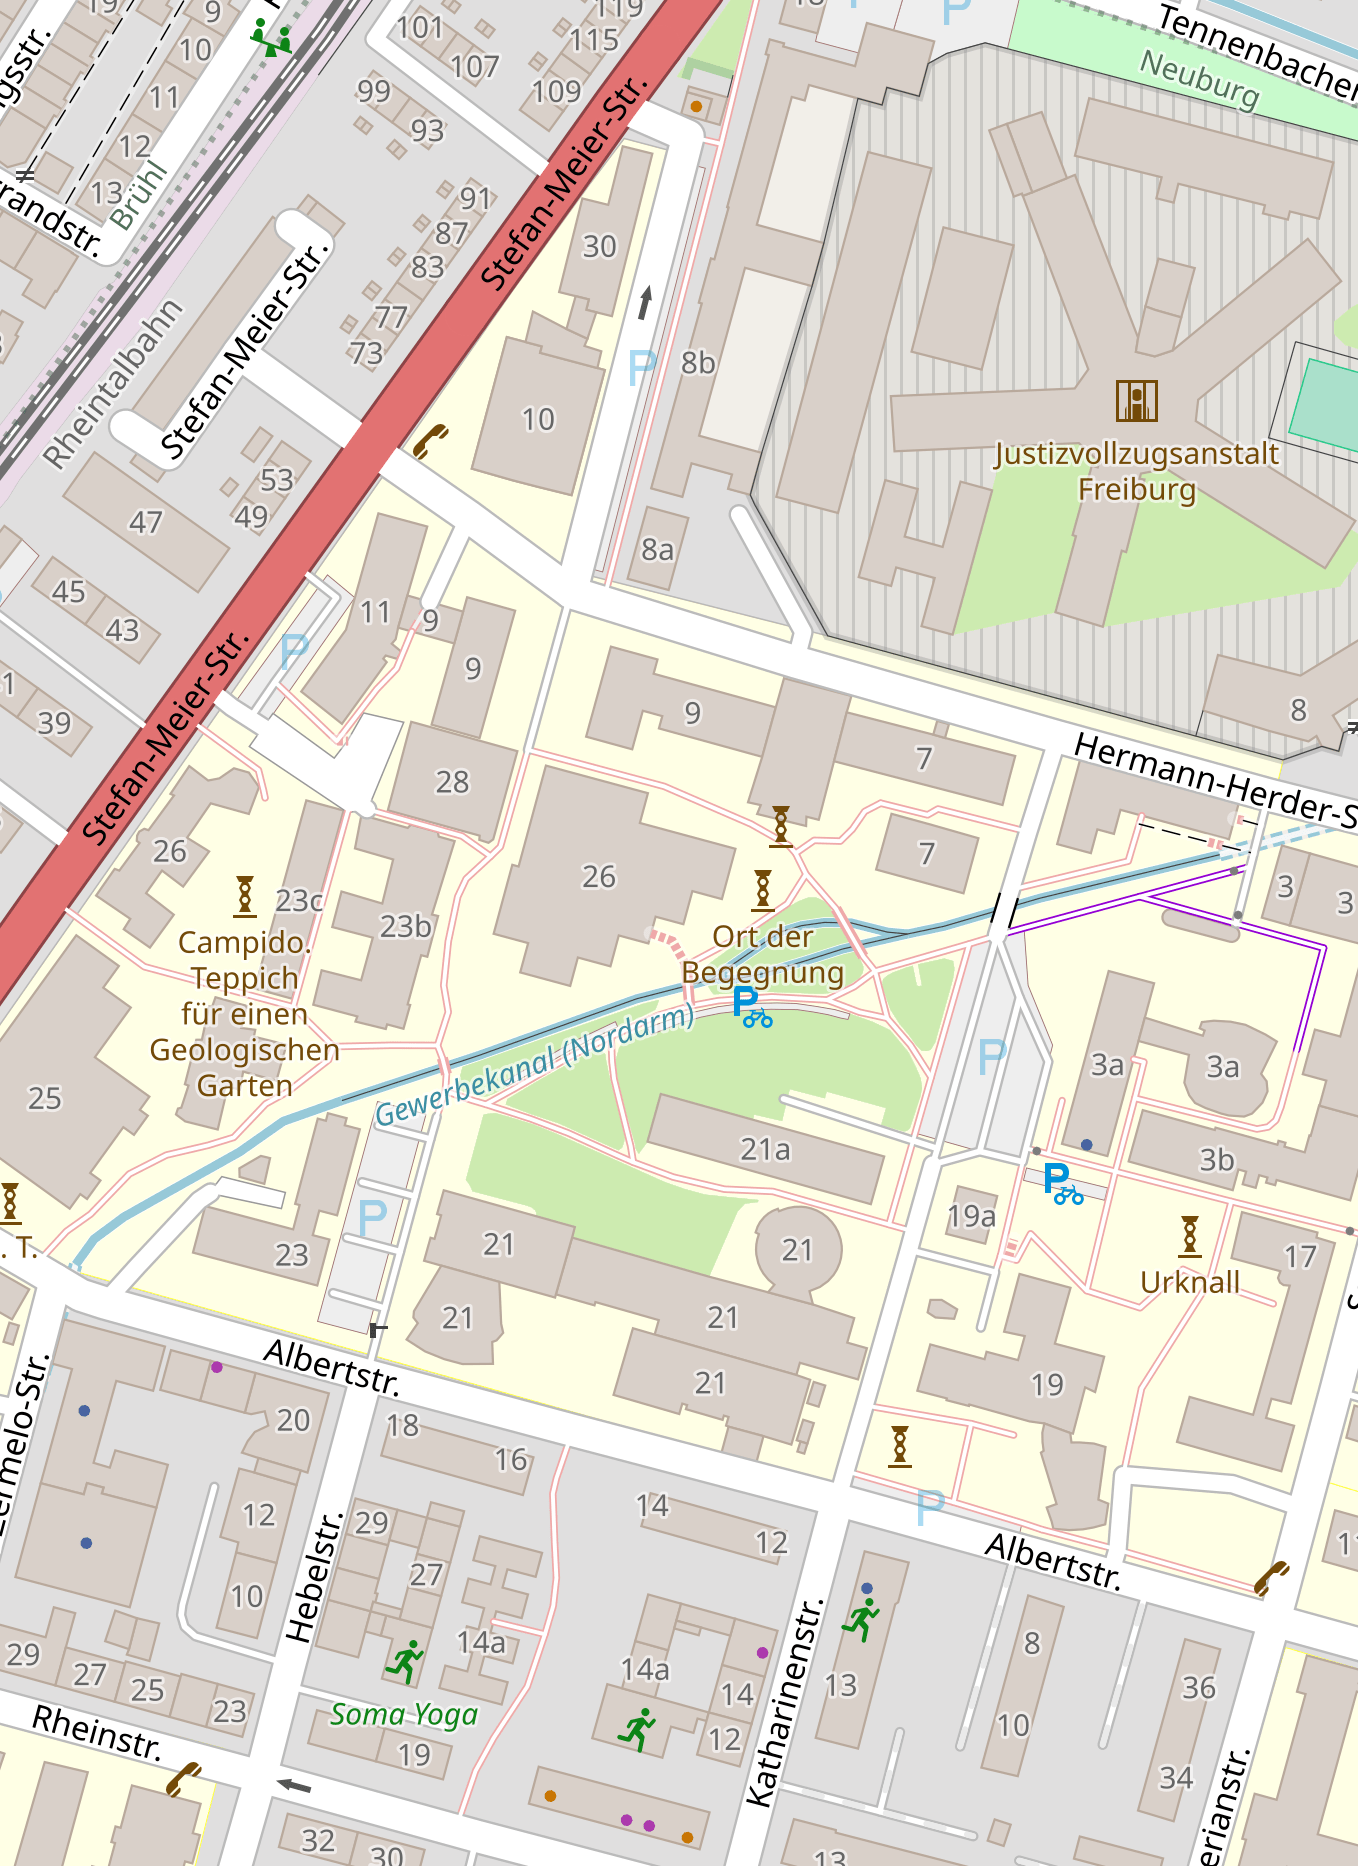
\includegraphics[width=115mm]{images-print/freiburg-campus.png}%
      };%
      % box for map key
      \fill [white] (0,39) rectangle (52,0);%
      % map key text
      \draw (8,8) node [anchor=south west, align=left] {%
        \begin{minipage}{47mm}%
          \small
          1 Hörsaal Rundbau \linebreak
          2 Ausstellung, Welcome Desk \linebreak
          3 Hörsaal Anatomie \linebreak
          4 Hörsaal Weismannhaus \linebreak
          5 Workshopräume \linebreak
          6 Hermann-Herder-Str. 9, R\,00\,020\linebreak
          7 Albertstr. 21, R\,00\,004\linebreak
          8 Mensa
        \end{minipage}%
      };
      % circles with numbers
      \node (1) at (67.00,49.50) [] {}; % HS Rundbau
      \node (1label) at (1) [fill=geoblau, draw=black, inner sep=0.3mm, circle] {1}; % HS Rundbau
      \node (2) at (64.00,40.00) [] {}; % Chemie-Hochhaus
      \node (2label) at (2) [fill=white, draw=black, inner sep=0.3mm, circle] {2}; % Chemie-Hochhaus
      \node (3) at (91.50,33.50) [] {}; % HS Anatomie
      \node (3label) at (3) [fill=hellgelb, draw=black, inner sep=0.3mm, circle] {3}; % HS Anatomie
      \node (4) at (69.50,59.00) [] {}; % HS Weismannhaus
      \node (4label) at (4) [fill=hellgruen, draw=black, inner sep=0.3mm, circle] {4}; % HS Weismannhaus
      \node (5) at (45.00,119.50) [] {}; % Workshopräume
      \node (5label) at (5) [fill=dezentrot, draw=black, inner sep=0.3mm, circle] {5}; % Workshopräume
      \node (6) at (55.00,98.50) [] {}; % BoF 1
      \node (6label) at (6) [fill=white, draw=black, inner sep=0.3mm, circle] {6}; % BoF 2
      \node (7) at (55.00,49.00) [] {}; % BoF 2
      \node (7label) at (7) [fill=white, draw=black, inner sep=0.3mm, circle] {7}; % BoF 2
      \node (8) at (51.00,87.00) [] {}; % Mensa
      \node (8label) at (8) [fill=white, draw=black, inner sep=0.3mm, circle] {8}; % Mensa
    \end{tikzpicture}%
  }%
]{campuskarte}
\newpairofpagestyles[]{page-campuskarte}{}
\AddLayersAtBeginOfPageStyle{page-campuskarte}{campuskarte}
\AddLayersAtBeginOfPageStyle{page-campuskarte}{cropmarksplain}
